\documentclass[10pt]{article}
\usepackage[utf8]{inputenc}\usepackage[T1]{fontenc}\usepackage{lmodern}
\usepackage[margin=1in]{geometry}
\usepackage{microtype}\setlength{\emergencystretch}{3em}
\usepackage{amsmath,amssymb,booktabs,graphicx,array,enumitem,caption}
\graphicspath{{figures/}}
\usepackage[round]{natbib}
\usepackage[hidelinks]{hyperref}
% AUTO-GENERATED by code/make_macros.py. Do not edit by hand.
% Every value traces to the results file named in the comment.
\makeatletter
\newcommand{\result}[1]{%
  \expandafter\ifx\csname result@#1\endcsname\relax
    \textbf{??}\PackageWarning{results}{undefined result key: #1}%
  \else\csname result@#1\endcsname\fi}
\newcommand{\defresult}[2]{\expandafter\def\csname result@#1\endcsname{#2}}
\makeatother

\defresult{ageFirstAttn}{0.117}   % results/attn_8L256_s0_coupling.json
\defresult{ageLastAttn}{0.166}   % results/attn_8L256_s0_coupling.json
\defresult{agePeakAttn}{0.387}   % results/attn_8L256_s0_coupling.json
\defresult{belIllAttn}{0.356}   % results/attn_8L256_s0_belief.json
\defresult{belIllHiAttn}{0.364}   % results/attn_8L256_s0_belief.json
\defresult{belIllLoAttn}{0.348}   % results/attn_8L256_s0_belief.json
\defresult{belLegAttn}{0.657}   % results/attn_8L256_s0_belief.json
\defresult{belMisAttn}{0.050}   % results/attn_8L256_s0_belief.json
\defresult{belRandAttn}{0.008}   % results/attn_8L256_s0_belief.json
\defresult{belRatioAttn}{44}   % results/attn_8L256_s0_belief.json
\defresult{belRatioMisAttn}{7.0}   % results/attn_8L256_s0_belief.json
\defresult{bestLayerAttn}{7.0}   % results/attn_8L256_s*.json
\defresult{bestLayerAttnN}{1}   % results/attn_8L256_s*.json
\defresult{bestLayerAttnSD}{0.0}   % results/attn_8L256_s*.json
\defresult{bestLayerBase}{7}   % results/attn_8L256_s0.json
\defresult{corrGlobalMaxAttn}{0.080}   % results/attn_8L256_s0_coupling.json
\defresult{corrGlobalMinAttn}{0.025}   % results/attn_8L256_s0_coupling.json
\defresult{ctlMaj40}{0.261}   % results/attn_8L256_s0.json
\defresult{exactPly}{0}   % results/attn_8L256_s0.json
\defresult{hill05Attn}{30}   % results/attn_8L256_s*.json
\defresult{hill05AttnN}{1}   % results/attn_8L256_s*.json
\defresult{hill05AttnSD}{0}   % results/attn_8L256_s*.json
\defresult{hill10Attn}{40}   % results/attn_8L256_s*.json
\defresult{hill10AttnN}{1}   % results/attn_8L256_s*.json
\defresult{hill10AttnSD}{0}   % results/attn_8L256_s*.json
\defresult{ill40Attn}{0.177}   % results/attn_8L256_s*.json
\defresult{ill40AttnN}{1}   % results/attn_8L256_s*.json
\defresult{ill40AttnSD}{0.000}   % results/attn_8L256_s*.json
\defresult{illFirst}{0.0004}   % results/attn_8L256_s0.json
\defresult{illLast}{0.319}   % results/attn_8L256_s0.json
\defresult{layerProfFirst}{0.322}   % results/attn_8L256_s0.json
\defresult{layerProfLast}{0.543}   % results/attn_8L256_s0.json
\defresult{locIllAttn}{0.806}   % results/attn_8L256_s0_coupling.json
\defresult{locLegAttn}{0.384}   % results/attn_8L256_s0_coupling.json
\defresult{massFirst}{0.993}   % results/attn_8L256_s0.json
\defresult{massLast}{0.455}   % results/attn_8L256_s0.json
\defresult{meanPly}{78.2}   % data/proc
\defresult{nGames}{120,000}   % data/proc
\defresult{nLayers}{8}   % results/attn_8L256_s0.json
\defresult{nVocab}{1,926}   % data/proc
\defresult{neval}{12,000}   % data/proc
\defresult{ntrainlm}{96,000}   % data/proc
\defresult{ntrainprobe}{12,000}   % data/proc
\defresult{occ40Attn}{0.559}   % results/attn_8L256_s*.json
\defresult{occ40AttnN}{1}   % results/attn_8L256_s*.json
\defresult{occ40AttnSD}{0.000}   % results/attn_8L256_s*.json
\defresult{occFirst}{0.974}   % results/attn_8L256_s0.json
\defresult{occLast}{0.063}   % results/attn_8L256_s0.json
\defresult{paramsAttn}{7,345,920}   % results/attn_8L256_s*.json
\defresult{patchAlphaAttn}{0.50}   % results/attn_8L256_s0_patch.json
\defresult{patchCutAttn}{0.934}   % results/attn_8L256_s0_patch.json
\defresult{patchDecAttn}{0.996}   % results/attn_8L256_s0_patch.json
\defresult{patchFlipAttn}{1.000}   % results/attn_8L256_s0_patch.json
\defresult{patchMassAfterAttn}{0.005}   % results/attn_8L256_s0_patch.json
\defresult{patchMassBeforeAttn}{0.071}   % results/attn_8L256_s0_patch.json
\defresult{patchNAttn}{700}   % results/attn_8L256_s0_patch.json
\defresult{patchRandAfterAttn}{0.065}   % results/attn_8L256_s0_patch.json
\defresult{patchRandCutAttn}{0.077}   % results/attn_8L256_s0_patch.json
\defresult{patchRandDecAttn}{0.484}   % results/attn_8L256_s0_patch.json
\defresult{synAccDeepAttn}{0.122}   % results/synth_attn_s*.json
\defresult{synAccDeepAttnN}{1}   % results/synth_attn_s*.json
\defresult{synAccDeepAttnSD}{0.000}   % results/synth_attn_s*.json
\defresult{synAccShallowAttn}{0.114}   % results/synth_attn_s*.json
\defresult{synAccShallowAttnN}{1}   % results/synth_attn_s*.json
\defresult{synAccShallowAttnSD}{0.000}   % results/synth_attn_s*.json
\defresult{synParamsAttn}{6,378,240}   % results/synth_attn_s*.json
\defresult{synPlanDeepAttn}{0.837}   % results/synth_attn_s*.json
\defresult{synPlanDeepAttnN}{1}   % results/synth_attn_s*.json
\defresult{synPlanDeepAttnSD}{0.000}   % results/synth_attn_s*.json
\defresult{synPlanShallowAttn}{0.813}   % results/synth_attn_s*.json
\defresult{synPlanShallowAttnN}{1}   % results/synth_attn_s*.json
\defresult{synPlanShallowAttnSD}{0.000}   % results/synth_attn_s*.json
\defresult{synStateDeepAttn}{0.964}   % results/synth_attn_s*.json
\defresult{synStateDeepAttnN}{1}   % results/synth_attn_s*.json
\defresult{synStateDeepAttnSD}{0.000}   % results/synth_attn_s*.json
\defresult{synStateShallowAttn}{0.966}   % results/synth_attn_s*.json
\defresult{synStateShallowAttnN}{1}   % results/synth_attn_s*.json
\defresult{synStateShallowAttnSD}{0.000}   % results/synth_attn_s*.json
\defresult{valAttn}{3.029}   % results/attn_8L256_s*.json
\defresult{valAttnN}{1}   % results/attn_8L256_s*.json
\defresult{valAttnSD}{0.000}   % results/attn_8L256_s*.json


\newif\ifanon
\ifdefined\ANON\anontrue\else\anonfalse\fi

\title{\bf Coherent Errors: Chess Transformers Play Correctly\\on Misremembered Boards}
\ifanon
  \author{\normalsize\itshape Anonymous submission}
\else
  \author{Mohit Pratap Singh Rathore \and Gunveer Sinh Kalsi \and Sriharsha Meduri\\
  \small Oviqo Private Limited}
\fi
\date{}

\begin{document}
\maketitle

\begin{abstract}
When a search-free chess transformer plays an illegal move, is it producing
noise, or acting correctly on a board it has misremembered? We answer this by
reading linear probes against a rules-engine oracle at every token, in models of
\result{paramsSmall} to \result{paramsLarge} parameters. Of the illegal moves a
model plays, \result{belIllAttn} are legal in the position its own probe says it
believes, against \result{belMisAttn} for the same move scored under another
position's belief and \result{belRandAttn} for an arbitrary illegal move, with a
decoding ceiling of \result{belLegAttn}. The belief is causally load-bearing:
editing the single probe direction that encodes an occupied square removes
\result{patchCutAttn} of the probability mass on moves from it, while a
norm-matched random edit removes \result{patchRandCutAttn} and shifts the mass at
chance. Both effects strengthen monotonically across a twelvefold range of model
size. We also find that where a world model is measured matters: whole-board
probe accuracy predicts an illegal next move at AUC \result{aucAggMin} to
\result{aucAggMax}, while the same representation restricted to the squares the
move uses reaches \result{aucActMin} to \result{aucActMax}, the two being
indistinguishable in the opening and separating with depth. Long-horizon failure
here is not noise breaking through. It is competent play in a world that has
drifted.
\end{abstract}

\section{Introduction}

A transformer stores nothing between positions. Every token's representation is
rebuilt from the whole prefix through attention \citep{vaswani2017attention}, so
any quantity a task requires exists only because the network re-derives it, at
every layer and every position. That re-derivation is dependable over short spans
and unreliable over long ones, and the usual remedies act outside the model:
tree search \citep{yao2023tree}, process supervision \citep{lightman2024lets},
sampling with a vote \citep{wang2023selfconsistency}. Each raises accuracy and
none says what fails inside.

The question matters because two candidate failures recommend opposite remedies.
If the model has forgotten the world, a verifier that rescores outputs pays
repeatedly to repair something the architecture gave away. If the model holds the
world and reasons badly over it, a verifier is exactly right. Telling them apart
requires reading an intermediate representation against a known-correct
intermediate state, and open-ended text has no such state.

Chess from move notation does, and that is why we use it: a rules engine gives
the exact position after any prefix, legality is decidable, and depth is
uniformly scaled. We are explicit that this buys measurement precision at the
cost of generality, and Section~\ref{sec:limits} states what it does not license.
Prior work established that such models carry board-state representations and
that intervening on them changes behaviour \citep{li2023emergent,
karvonen2024emergent, toshniwal2022chess}. We take that as premise. Our question
is what happens to those representations as reasoning deepens, and whether their
failures explain the model's failures.

\paragraph{Findings.}
\begin{enumerate}[nosep,leftmargin=*]
\item \textbf{The errors are coherent.} \result{belIllAttn} of illegal moves are
legal in the model's own decoded board, against \result{belMisAttn} for a
mismatched belief and \result{belRandAttn} for a random illegal move.
\item \textbf{The belief is read, not merely present.} A calibrated edit to one
probe direction removes \result{patchCutAttn} of the mass on moves from the
affected square; a norm-matched random edit removes \result{patchRandCutAttn}.
\item \textbf{Where the world model is measured matters, increasingly with
depth.} Aggregate probe accuracy predicts illegality at AUC \result{aucAggMin} to
\result{aucAggMax}; restricted to the squares the move uses,
\result{aucActMin} to \result{aucActMax}.
\end{enumerate}

\section{Setup}
\label{sec:setup}

\paragraph{Data and oracle.} \result{nGames} human games above a rating floor,
deduplicated and split \emph{by game} so no prefix is shared between probe
fitting and evaluation: \result{ntrainlm} for training, \result{ntrainprobe} for
probes, \result{neval} for evaluation, mean length \result{meanPly} plies. A
rules engine emits the exact state after every token. Models are decoder-only,
trained on move notation alone, with no search at inference.

\paragraph{Probes and controls.} One linear head per layer predicting per-square
occupancy, fitted on the probe split and reported on the evaluation split.
Because most squares are empty, we report accuracy on occupied squares against
three controls: a per-square per-depth majority predictor, a label-permutation
control that pairs activations with another game's state at equal depth, and a
randomised-weight model of identical architecture
(Table~\ref{tab:controls}, following \citealp{hewitt2019designing}).

\paragraph{Observables.} State-tracking error is observed behaviourally as the
rate at which the model's top-1 move is illegal in the true position, and
representationally as probe-oracle disagreement.

\section{Results}

\subsection{State and behaviour decay together}

\begin{table}[t]
\centering\small
\caption{State decodability against every trivial explanation, for the
baseline model. Occupied-square accuracy at the most decodable layer,
beside a per-square per-depth majority predictor, a label-permutation
control, and a randomised-weight model of identical architecture. The gap
is what training put there.}
\label{tab:controls}
\begin{tabular}{lccccc}
\toprule
Ply & model & majority & label perm. & random weights & illegal rate \\
\midrule
0--10 & 0.975 & 0.867 & 0.879 & 0.898 & 0.0004 \\
10--20 & 0.876 & 0.599 & 0.673 & 0.641 & 0.0115 \\
20--30 & 0.761 & 0.444 & 0.487 & 0.439 & 0.0439 \\
30--40 & 0.655 & 0.359 & 0.315 & 0.297 & 0.0982 \\
40--50 & 0.557 & 0.261 & 0.166 & 0.195 & 0.1766 \\
50--60 & 0.475 & 0.073 & 0.072 & 0.141 & 0.2347 \\
60--80 & 0.353 & 0.000 & 0.019 & 0.071 & 0.2920 \\
80--120 & 0.173 & 0.000 & 0.001 & 0.038 & 0.3231 \\
120--161 & 0.066 & 0.000 & 0.000 & 0.030 & 0.3192 \\
\bottomrule
\end{tabular}
\end{table}


Occupied-square decodability falls from \result{occFirst} in the opening to
\result{occLast} in the deepest bucket, while the illegal top-1 rate rises from
\result{illFirst} to \result{illLast} and the mass on legal moves falls from
\result{massFirst} to \result{massLast} (Figure~\ref{fig:decay}). At mid-game the
trained model is clear of every trivial explanation, \result{occ40Attn} against
\result{ctlMaj40} for the majority predictor. There is a real state
representation, and it is being lost.

\begin{figure}[t]
\centering
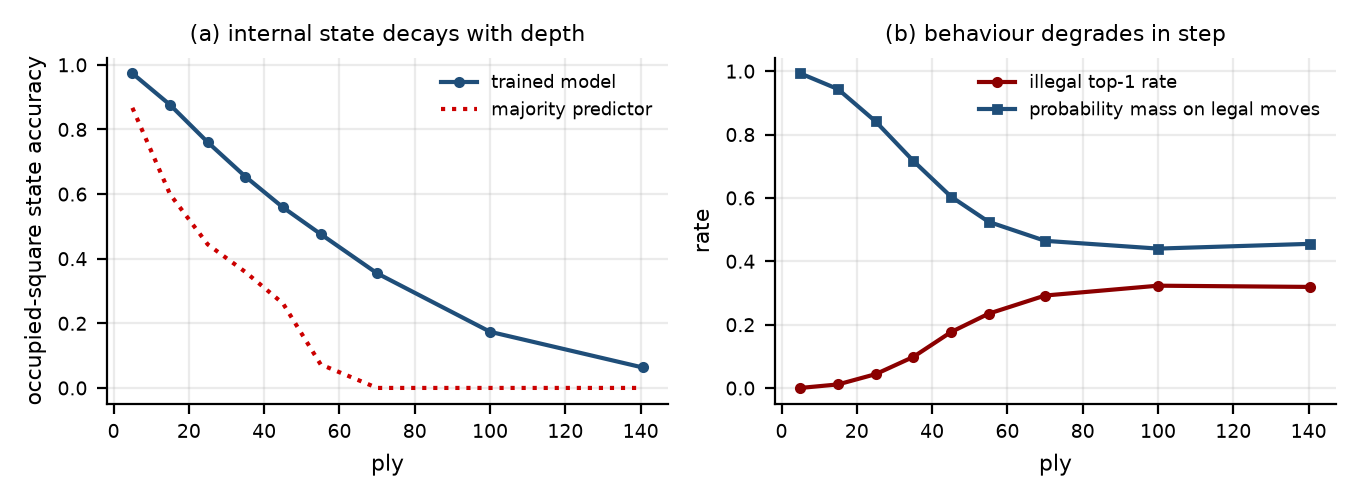
\includegraphics[width=\linewidth]{decay.png}
\caption{Internal state and external behaviour decay together. (a) Occupied-square
accuracy against three controls. (b) Illegal top-1 rate and the probability mass
on legal continuations.}
\label{fig:decay}
\end{figure}

\subsection{Where the world model is measured matters}

Two curves falling together is not evidence that one causes the other. We score
aggregate and action-relevant state error identically, as predictors of the same
binary outcome on the same samples, within depth so neither can simply track
depth (Table~\ref{tab:auc}).

\begin{table}[t]
\centering\small
\caption{Aggregate and action-relevant state error compared like for
like, as predictors of the same binary outcome on the same samples:
whether the model's top-1 move is illegal. AUC is computed within each
depth bucket so neither predictor can simply be tracking depth. The
standardised coefficients come from a logistic fit containing both
predictors. The aggregate measure is informative and it is the weaker of
the two, and the gap widens with depth.}
\label{tab:auc}
\begin{tabular}{lccccr}
\toprule
Ply & AUC aggregate & AUC action-relevant & $\beta$ aggregate & $\beta$ action-relevant & $n$ \\
\midrule
10--20 & 0.671 & \textbf{0.687} & +0.065 & \textbf{+0.153} & 15{,}000 \\
20--30 & 0.627 & \textbf{0.681} & +0.120 & \textbf{+0.332} & 15{,}000 \\
30--40 & 0.584 & \textbf{0.662} & +0.100 & \textbf{+0.506} & 14{,}511 \\
40--50 & 0.548 & \textbf{0.643} & +0.057 & \textbf{+0.573} & 13{,}176 \\
50--60 & 0.551 & \textbf{0.617} & +0.114 & \textbf{+0.500} & 11{,}262 \\
60--80 & 0.538 & \textbf{0.592} & +0.076 & \textbf{+0.431} & 16{,}426 \\
\midrule
pooled, depth as covariate & n/a & n/a & +0.118 & \textbf{+0.504} & 85{,}375 \\
\bottomrule
\end{tabular}
\end{table}


Aggregate board fidelity predicts an illegal move at AUC \result{aucAggMin} to
\result{aucAggMax}, which is above chance and not negligible. The same
representation restricted to the two squares the move touches reaches
\result{aucActMin} to \result{aucActMax}. In the opening the two are nearly
indistinguishable; the gap opens with depth, and in a joint fit the
action-relevant term carries a standardised weight of \result{betaAct} against
\result{betaAgg}. Whole-board probe accuracy, the quantity usually reported as
evidence of a world model, is a usable but weak proxy for whether that model is
load-bearing, and it weakens exactly where long-horizon behaviour matters.

\subsection{The errors are coherent}
\label{sec:belief}

If state loss drives the failure, an invalid action should be valid in the state
the model believes it is in. We reconstruct that believed position from the
probe, clearing castling rights so nothing is licensed by an assumption we did
not decode, and test pseudo-legality because a decoded board may lack a king.

\begin{table}[t]
\centering\small
\caption{Does state loss explain behaviour? Aggregate error is the
within-depth correlation between misremembered squares and playing an
illegal move. Action-relevant error is the probability the probe is wrong
on the squares the move uses. Belief consistency is the share of illegal
moves that are legal in the model's own decoded board, beside the same
move under another position's belief, an arbitrary illegal move, and the
decoding ceiling given by genuinely legal moves.}
\label{tab:mechanism}
\begin{tabular}{lrccccccc}
\toprule
& & aggregate & \multicolumn{2}{c}{action-relevant} & \multicolumn{4}{c}{belief consistency} \\
\cmidrule(lr){4-5}\cmidrule(lr){6-9}
Model & Params & corr. & illegal & legal & own & mismatch & random & ceiling \\
\midrule
Attention-only & 7{,}345{,}920 & 0.02 to 0.08 & 0.806 & 0.384 & \textbf{0.356} & 0.050 & 0.008 & 0.657 \\
Attention-only, parameter-matched & 7{,}505{,}976 & 0.01 to 0.10 & 0.804 & 0.391 & \textbf{0.350} & 0.051 & 0.007 & 0.650 \\
Recurrent channel ($\lambda{=}0$) & 7{,}508{,}416 & 0.03 to 0.12 & 0.801 & 0.384 & \textbf{0.358} & 0.053 & 0.007 & 0.658 \\
Recurrent channel ($\lambda{=}1$) & 7{,}508{,}416 & -0.05 to 0.08 & 0.806 & 0.399 & \textbf{0.366} & 0.093 & 0.021 & 0.656 \\
6L/192 & 3{,}440{,}064 & 0.01 to 0.10 & 0.831 & 0.447 & \textbf{0.266} & 0.049 & 0.006 & 0.581 \\
12L/384 & 22{,}835{,}328 & -0.02 to 0.07 & 0.747 & 0.327 & \textbf{0.412} & 0.056 & 0.009 & 0.713 \\
12L/512 & 39{,}884{,}288 & -0.04 to 0.07 & 0.711 & 0.297 & \textbf{0.439} & 0.059 & 0.009 & 0.745 \\
\bottomrule
\end{tabular}
\end{table}


Of the illegal moves the model plays, \result{belIllAttn} are legal in its own
believed position, with a bootstrap interval of [\result{belIllLoAttn},
\result{belIllHiAttn}]. Two controls bound the alternatives. The same move scored
against a believed position decoded elsewhere at equal depth is legal
\result{belMisAttn} of the time, so the effect is specific to this belief at this
position rather than to plausible boards generally. An arbitrary illegal move
scored against the model's own believed position is legal \result{belRandAttn} of
the time, so the believed board is not permissive. The ceiling on what this test
can detect is \result{belLegAttn}, the rate at which genuinely legal moves are
recovered, which is below one because probe decoding is lossy.

\begin{figure}[t]
\centering
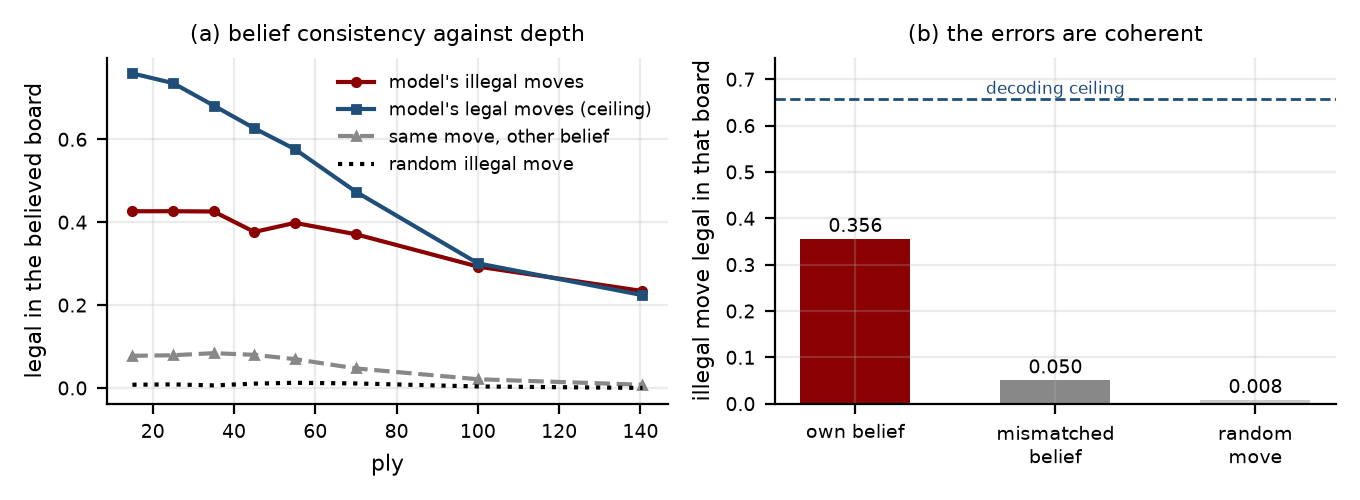
\includegraphics[width=\linewidth]{belief.png}
\caption{(a) Belief consistency against depth, restricted to buckets with at
least thirty illegal cases. (b) Pooled, with the decoding ceiling marked.}
\label{fig:belief}
\end{figure}

\subsection{Inducing a false belief changes the action}
\label{sec:causal}

The result above is observational. We therefore intervene: at a position where
the side to move genuinely occupies a square, we push the residual stream along
the probe direction encoding ``this square is empty'' and ask whether the model
stops proposing moves from it.

Edit strength must be calibrated rather than chosen, because a large enough push
degrades the forward pass and moves behaviour for reasons unrelated to belief.
Below a quarter of the residual-stream magnitude the edit does not reliably flip
the decoded belief; above roughly one, the norm-matched random control also
destroys the output distribution. We report at \result{patchAlphaAttn}, inside
that window (Figure~\ref{fig:patchcal}).

\begin{table}[t]
\centering\small
\caption{Causal intervention at the calibrated edit strength. Editing the
state direction removes probability mass from moves out of the affected
square; a norm-matched random direction does not. The manipulation check
reports how often the edit actually changed the decoded belief.}
\label{tab:patch}
\begin{tabular}{lccccc}
\toprule
Model & $n$ & belief flipped & mass before & mass after & random edit after \\
\midrule
Attention-only & 700 & 1.000 & 0.071 & \textbf{0.005} & 0.065 \\
Attention-only, parameter-matched & 600 & 1.000 & 0.074 & \textbf{0.004} & 0.066 \\
Recurrent channel ($\lambda{=}0$) & 600 & 1.000 & 0.070 & \textbf{0.004} & 0.064 \\
Recurrent channel ($\lambda{=}1$) & 600 & 1.000 & 0.067 & \textbf{0.004} & 0.062 \\
\bottomrule
\end{tabular}
\end{table}


At that strength the manipulation check succeeds in \result{patchFlipAttn} of
cases, the state edit removes \result{patchCutAttn} of the probability mass on
moves from the affected square, and the norm-matched random edit removes
\result{patchRandCutAttn} while changing the mass in \result{patchRandDecAttn} of
cases, which is a coin flip. The state representation is read.

\begin{figure}[t]
\centering
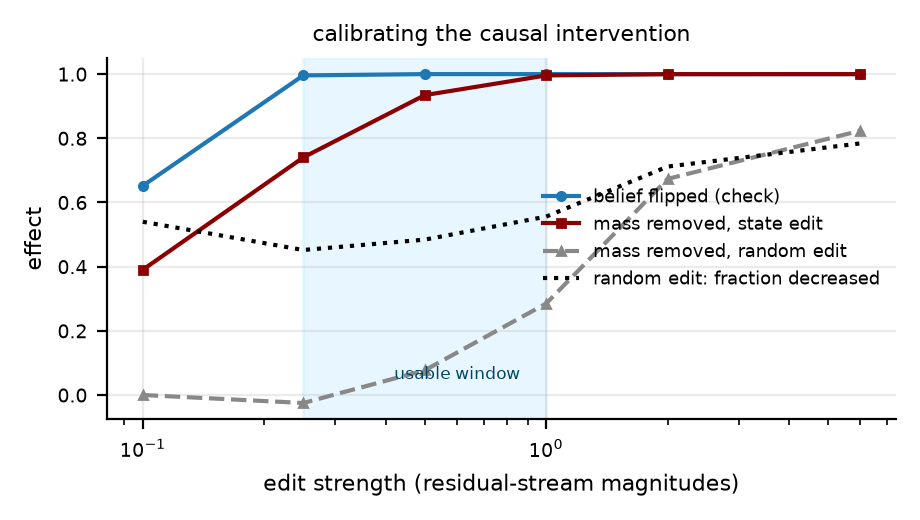
\includegraphics[width=0.62\linewidth]{patch_calibration.png}
\caption{Calibrating the intervention. Too small and the belief does not flip;
too large and a random direction also destroys the output. We report inside the
shaded window.}
\label{fig:patchcal}
\end{figure}

\subsection{Both effects strengthen with scale}

\begin{table}[t]
\centering\small
\caption{The scale ladder, three seeds per rung. $H_{\mathrm{ill}}$ is read
off behaviour, the ply at which the illegal-move rate crosses five percent.
$H_{\mathrm{fid}}$ is read off the representation, the depth at which the
probe first fails on the squares the chosen move touches more than half the
time, and so cannot be moved by hedging. Belief consistency is normalised by
each model's own legal-move recovery reference, because that reference rises with
size. Mean\,$\pm$\,s.d.\ over seeds.}
\label{tab:scale}
\begin{tabular}{lrccccc}
\toprule
Model & Params & seeds & $H_{\mathrm{ill}}(.05)$ & $H_{\mathrm{fid}}(.5)$ & belief\,/\,reference & mismatch \\
\midrule
6L/192 & 3{,}440{,}064 & 3 & 21.4\,$\pm$\,0.1 & 33.8\,$\pm$\,0.2 & 0.476\,$\pm$\,0.017 & 0.051\,$\pm$\,0.002 \\
8L/256 & 7{,}345{,}920 & 3 & 26.1\,$\pm$\,0.0 & 40.8\,$\pm$\,0.5 & 0.534\,$\pm$\,0.008 & 0.052\,$\pm$\,0.002 \\
12L/256 & 10{,}504{,}960 & 3 & 27.8\,$\pm$\,0.2 & 42.1\,$\pm$\,0.3 & 0.552\,$\pm$\,0.007 & 0.051\,$\pm$\,0.002 \\
8L/384 & 15{,}737{,}472 & 3 & 29.5\,$\pm$\,0.2 & 50.0\,$\pm$\,0.4 & 0.568\,$\pm$\,0.008 & 0.053\,$\pm$\,0.001 \\
12L/384 & 22{,}835{,}328 & 3 & 31.7\,$\pm$\,0.3 & 52.5\,$\pm$\,0.5 & 0.577\,$\pm$\,0.005 & 0.053\,$\pm$\,0.003 \\
12L/512 & 39{,}884{,}288 & 3 & 33.8\,$\pm$\,0.1 & 59.1\,$\pm$\,0.5 & 0.587\,$\pm$\,0.011 & 0.056\,$\pm$\,0.004 \\
\bottomrule
\end{tabular}
\end{table}


Across six rungs from \result{paramsSmall} to \result{paramsLarge} parameters,
three seeds each, belief consistency normalised by each model's own decoding
ceiling rises monotonically from \result{belRatioNRung1} to
\result{belRatioNRung6}, while the mismatched control stays flat
(Figure~\ref{fig:scale}). The mechanism is not an artifact of the smallest
models: larger models make a \emph{larger} fraction of their errors coherently.

\begin{figure}[t]
\centering
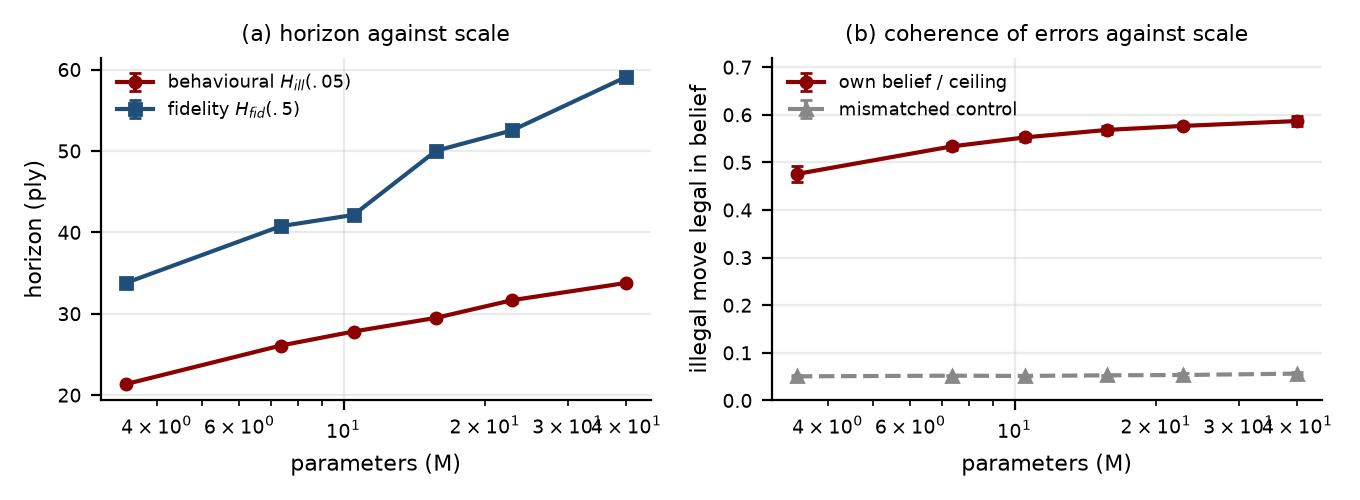
\includegraphics[width=\linewidth]{scale.png}
\caption{(a) Both horizons against scale. (b) Belief consistency normalised by
each model's decoding ceiling, with its matched control. Three seeds per rung.}
\label{fig:scale}
\end{figure}

\paragraph{A horizon that does not depend on behaviour.}
Behavioural horizons are fragile: ablating the recurrent read-out of a variant
model \emph{lowers} its illegal-move rate while \emph{raising} its language-model
loss, because the ablated model hedges toward the legal-move prior
(Appendix). We therefore also define $H_{\mathrm{fid}}$, the depth at which the
probe first fails on the squares the chosen move touches more than half the time.
It never consults the output distribution, so hedging buys nothing. It runs from
\result{hfidRung1} to \result{hfidRung6} ply across the ladder against
\result{hintRung1} to \result{hintRung6} for the behavioural horizon, ordering
the models identically.

\section{What failed}

Four results went against us and are reported where they changed a decision. We
predicted state would be most decodable mid-stack; it is maximal at the final
block, rising from \result{layerProfFirst} to \result{layerProfLast}. Our
pre-registered horizon, defined on exact-position fidelity, is degenerate: that
quantity is zero past ply \result{exactPly} in every condition. An auxiliary
state objective raises probe accuracy to the level of a model twice the size,
\result{occ40AlsbOne} against \result{occ40AttnWide}, while buying a small
fraction of its behavioural gain. And a second oracle-bearing domain took seven
designs to reach a measurable regime, then failed to replicate for its
attention-only condition, because the task permits resolving one queried object
on demand rather than maintaining state. All four are detailed in the appendix.

\section{Discussion and limitations}
\label{sec:limits}

The practical content is a change in what to measure. Reporting that a probe
recovers a world model at some aggregate accuracy is weak evidence that the model
is load-bearing; the same representation scored on the state an action consumes
is substantially more informative, increasingly so with depth. Any team
instrumenting a system for long-horizon reliability should condition on the state
the action uses.

The belief-consistency result also reframes the failure. A model that plays a
coherent move in a misremembered position is not behaving erratically, and
treatments assuming erratic behaviour aim at the wrong target: sampling several
chains and voting will not help if every chain is drawn from the same drifted
state.

\paragraph{What this does not show.} Our models span \result{paramsSmall} to
\result{paramsLarge} parameters in a single domain. We make no claim about
frontier-scale systems or about natural language, and the natural-language
transfer test is absent rather than approximated. Probe decoding is lossy, which
is why the ceiling is reported rather than assumed; belief consistency is tested
with pseudo-legal moves, which the random-move control is designed to bound. The
strongest available next test is a domain with an exact oracle that is neither
chess nor constructed as a benchmark, and we argue program execution traces are
that domain.

\section{Conclusion}

Measured against an exact oracle, long-horizon failure in these models separates
into memory and judgement, and the memory component behaves in a specific and
somewhat unsettling way. The model does not degrade into noise. It plays a
reasonable move in a board it has misremembered, and it does so more consistently
as it gets larger.


\appendix
\section{The intervention we evaluated with the diagnostic}
\label{app:alsb}

To test whether the diagnostic discriminates between architectures, we trained a
variant with a fixed-width gated recurrent channel inserted after every $k$-th
attention block, carrying $z_t \in \mathbb{R}^{d_s}$ with $d_s \ll d$, read back
into the residual stream, with an optional auxiliary loss supervising $z_t$ to be
the state. Architecture, supervision and read-out are varied independently
against a parameter-matched attention-only control.

\begin{table}[t]
\centering\small
\caption{Horizon and state fidelity by condition. $H_{\mathrm{ill}}(.05)$ is
the ply at which the illegal-move rate first crosses five percent,
interpolated between bucket midpoints because the bucketed read-off returns
the same bucket for every condition and so discriminates nothing.
Mean\,$\pm$\,s.d.\ over seeds where more than one was run.}
\label{tab:horizon}
\begin{tabular}{lrcccc}
\toprule
Model & Params & seeds & occ.\ acc.\ @40--50 & illegal @40--50 & $H_{\mathrm{ill}}(.05)$ \\
\midrule
Attention-only & 7{,}345{,}920 & 3 & 0.555\,$\pm$\,0.003 & 0.176\,$\pm$\,0.002 & 26.1\,$\pm$\,0.0 \\
Attention-only, parameter-matched & 7{,}505{,}976 & 3 & 0.554\,$\pm$\,0.002 & 0.172\,$\pm$\,0.003 & 26.0\,$\pm$\,0.1 \\
Recurrent channel ($\lambda{=}0$) & 7{,}508{,}416 & 3 & 0.556\,$\pm$\,0.003 & 0.169\,$\pm$\,0.002 & 26.2\,$\pm$\,0.3 \\
Recurrent channel ($\lambda{=}1$) & 7{,}508{,}416 & 3 & 0.632\,$\pm$\,0.003 & 0.166\,$\pm$\,0.002 & 26.5\,$\pm$\,0.2 \\
\midrule
\quad read-out ablated at test & n/a & 3 & 0.559\,$\pm$\,0.005 & 0.149\,$\pm$\,0.005 & 27.2\,$\pm$\,0.4 \\
\midrule
\quad 6L/192 & 3{,}440{,}064 & 3 & 0.468\,$\pm$\,0.006 & 0.245\,$\pm$\,0.003 & 21.4\,$\pm$\,0.1 \\
\quad 8L/256 & 7{,}345{,}920 & 3 & 0.555\,$\pm$\,0.003 & 0.176\,$\pm$\,0.002 & 26.1\,$\pm$\,0.0 \\
\quad 12L/256 & 10{,}504{,}960 & 3 & 0.577\,$\pm$\,0.005 & 0.149\,$\pm$\,0.001 & 27.8\,$\pm$\,0.2 \\
\quad 8L/384 & 15{,}737{,}472 & 3 & 0.632\,$\pm$\,0.006 & 0.134\,$\pm$\,0.004 & 29.5\,$\pm$\,0.2 \\
\quad 12L/384 & 22{,}835{,}328 & 3 & 0.656\,$\pm$\,0.001 & 0.112\,$\pm$\,0.002 & 31.7\,$\pm$\,0.3 \\
\quad 12L/512 & 39{,}884{,}288 & 3 & 0.694\,$\pm$\,0.003 & 0.101\,$\pm$\,0.001 & 33.8\,$\pm$\,0.1 \\
\bottomrule
\end{tabular}
\end{table}


With the auxiliary objective active, state decodability rises sharply, from
\result{occ40Attn} to \result{occ40AlsbOne} at matched parameters and tokens. The
architecture without the objective, \result{occ40AlsbZero}, is indistinguishable
from baseline. Behaviour barely follows: the illegal rate improves from
\result{ill40Attn} to \result{ill40AlsbOne} and the horizon from
\result{hintAttn} to \result{hintAlsbOne} ply, while a plain attention model of
twice the size reaches almost the same decodability, \result{occ40AttnWide}, and
converts it into a much larger behavioural gain. An auxiliary loss that makes
state linearly available does what it is asked; being available is not being
used.

\paragraph{An ablation that improves behaviour.} Zeroing the read-out at test
time lowers the illegal rate, from \result{ill40AlsbOne} to \result{ill40Zab},
and lengthens the horizon. Language-model loss rises when it is removed, from
\result{lmIntact} to \result{lmAblated} across seeds, and the read-out injects a
vector of \result{injRatio} of the residual stream's norm, so it is not
vestigial. The ablated model is worse at prediction and better at staying legal
because it places more mass on legal moves, \result{massAblated} against
\result{massIntact}, while committing less to any one. The illegal rate is
therefore not a monotone proxy for state quality, which is why we also report
$H_{\mathrm{fid}}$.

\section{How much of the planning error is really memory}
\label{app:plan}

The conditioning that would isolate judgement cleanly is unattainable: requiring
the probe to recover the exact board leaves no samples past the opening.
Requiring only the squares the move touches leaves samples everywhere but does
not constrain the rest of the board. We therefore vary the strictness.

\begin{table}[t]
\centering\small
\caption{Planning error against how strictly we condition on state. Each
cell gives the median engine centipawn loss, the blunder rate, and the
sample size, over legal moves whose touched squares the probe recovers and
with at most the stated number of other squares wrong. Tightening the
conditioning lowers the loss, so part of what looks like degraded judgement
is state loss elsewhere on the board. Loss still grows with depth at fixed
conditioning, so part of it is not. Cells with fewer than thirty scored
positions are reported as n/a, and that scarcity is itself the finding:
at depth a nearly intact board is rare.}
\label{tab:strict}
\begin{tabular}{lcccccc}
\toprule
Ply & $\leq 0$ & $\leq 2$ & $\leq 4$ & $\leq 8$ & $\leq 16$ & any \\
\midrule
20--30 & n/a & 24 / 0.18 (115) & 24 / 0.21 (300) & 31 / 0.22 (300) & 44 / 0.31 (300) & 58 / 0.34 (300) \\
30--40 & n/a & n/a & 38 / 0.25 (85) & 62 / 0.36 (300) & 75 / 0.41 (300) & 91 / 0.47 (300) \\
40--50 & n/a & n/a & n/a & 67 / 0.41 (300) & 120 / 0.53 (300) & 111 / 0.52 (300) \\
\bottomrule
\end{tabular}
\end{table}


Tightening lowers the loss substantially: at ply 30 to 40 the median centipawn
loss falls from \result{epsMed30to40tol64} with the board unconstrained to
\result{epsMed30to40tol4} when at most four other squares may be wrong, and the
blunder rate from \result{epsBl30to40tol64} to \result{epsBl30to40tol4}. Roughly
half of what a naive reading calls degraded judgement is misattributed memory
failure. It does not go to zero: at fixed conditioning the loss still grows with
depth, from \result{epsMed20to30tol4} to \result{epsMed30to40tol4}. Memory is the
dominant component and not the only one.

\section{A second domain, and why it did not replicate}
\label{app:boxes}

We attempted a second oracle-bearing domain. Four arithmetic designs floored
because they required modular arithmetic before state tracking became visible;
training loss sat at the generator's token-type entropy, the value a model
reaches by learning the format and nothing else. A fifth, permutation tracking
over five objects, also floored, and instructively: with five objects the state
is an element of $S_5$, the smallest non-solvable symmetric group, which is
precisely the case bounded-depth models are known to be unable to track
\citep{merrill2024illusion}. Four objects give the solvable $S_4$. A sixth was
all-or-nothing, admitting no partial credit; querying after every operation
supplies it.

\begin{table}[t]
\centering\small
\caption{Domain 2, permutation tracking. Answer accuracy at the shallowest
and deepest depths against a chance rate of one in four, the probe's
recovery of the queried object at depth, and belief consistency beside its
mismatched control. The attention-only model solves the task well above
chance while its state stays at chance under the probe, so it is not
maintaining a linearly decodable assignment. The supervised channel is, and
its errors are coherent with it.}
\label{tab:boxes}
\begin{tabular}{lccccc}
\toprule
Model & seeds & acc.\ shallow & acc.\ deep & probe deep & belief / control \\
\midrule
Attention-only & 3 & 1.000\,$\pm$\,0.000 & 0.589\,$\pm$\,0.010 & 0.263\,$\pm$\,0.010 & 0.256\,$\pm$\,0.005 / 0.249\,$\pm$\,0.003 \\
Recurrent channel ($\lambda{=}1$) & 3 & 1.000\,$\pm$\,0.000 & 0.989\,$\pm$\,0.001 & 0.983\,$\pm$\,0.001 & 0.701\,$\pm$\,0.017 / 0.254\,$\pm$\,0.009 \\
\bottomrule
\end{tabular}
\end{table}


The seventh design is measurable, and the outcome is not a replication. With the
supervised channel the task is nearly solved at every depth and belief
consistency reproduces, \result{beliefBoxAlsb} against a mismatched control of
\result{beliefMisBoxAlsb}. The attention-only model solves the task well above
chance, \result{ansDeepBoxAttn} at depth, while its probe recovers state at
\result{probeDeepBoxAttn}, which is chance. The same probe procedure recovers
\result{probeDeepBoxAlsb} in the other model, so this is a fact about the model.
The task permits resolving one queried object on demand by tracing its history,
so it never obliges the model to maintain an assignment. Chess allows no such
shortcut. A task can carry an exact oracle, be learnable, and still fail to
measure state maintenance.

\bibliographystyle{apalike}
\bibliography{refs}

\end{document}
